\documentclass[10pt]{report}

\usepackage{subcaption} % for subfigures
\usepackage{amsthm} % for QED
%\usepackage{algpseudocode} % for pseudo-code
\usepackage{mathtools} % for delimiter

\usepackage{listings} % for code
\lstset
{
	language=Matlab,
	frame=single,
	basicstyle=\footnotesize,
	captionpos=b,
	numbers=left,
	stepnumber=1,
	showstringspaces=false,
	tabsize=4,
	breaklines=true,
	breakatwhitespace=false,
}

\usepackage{float} % for figure [H]
\usepackage{booktabs} % for tabular
\usepackage{caption} % for \caption*
\usepackage[export]{adjustbox} % for valign=t
\usepackage{array} % for column type m
\usepackage{verbatim}
\usepackage{graphicx}
\graphicspath{ {imgs/} }
\usepackage{fancyhdr}
\usepackage{amssymb}
\usepackage{amsmath}

%%%%%% Pagination
\setlength{\topmargin}{-.3 in}
\setlength{\oddsidemargin}{0in}
\setlength{\evensidemargin}{0in}
\setlength{\textheight}{9.in}
\setlength{\textwidth}{6.5in}

%Title page
\newcommand{\hwTitle}{Homework \#5}
\newcommand{\hwCourse}{Numerical Differential Equations/Computational Mathematics II}
\newcommand{\hmwkClassInstructor}{Professor Shuwang Li}

\title{
	\vspace{2in}
	\textmd{\textbf{\hwCourse\\\hwTitle}}\\
	\vspace{0.3in}\large{\textit{\hmwkClassInstructor}}
	\vspace{3in}
}

%\title{Homework 1}
\author{\textbf{Zhihao Ai}}
\date{}

%Header setting. 
\pagestyle{fancy}
\fancyhead[L]{Zhihao Ai}
\fancyhead[C]{Math 478}
\fancyhead[R]{Homework 5}
%%%%%%

%Global setting.
%\everymath{\displaystyle}
\setlength\parindent{0pt}

%Custom general commands.
\newcommand{\ds}{\displaystyle}
\newcommand{\ts}{\textstyle}
\newcommand{\f}[1] {f\left(#1\right)}
\newcommand{\eva}[2] {\left. #1 \right|_{#2}}
\newcommand{\dintt}[4] {\int_{#1}^{#2} #3 d#4}

\newcolumntype{N}{ >$ c <$}
\newcolumntype{M}[1]{>{\centering\arraybackslash $}m{#1}<{$}}

\newcommand{\abs}[1] {\left| #1 \right|}

\DeclarePairedDelimiter\autoparen{(}{)}
\newcommand{\pa}[1]{\autoparen*{#1}}
\DeclarePairedDelimiter\autodvert{\Vert}{\Vert}
\DeclarePairedDelimiter{\floor}{\lfloor}{\rfloor}
\newcommand{\norm}[1]{\autodvert*{#1}}

\begin{document}

\maketitle

\section*{Question 1}
% Fundamental concepts on Runge-Kutta methods.
\begin{enumerate}
	\item 
	(Problem 3.2) Let us define
	\[
	T_n(\cos{\theta}) := \cos{n\theta},\quad n = 0,1,2,\dots, \quad -\pi\le \theta\le \pi.
	\]
	\begin{enumerate}
		\item 
		Show that each $T_n$ is a polynomial of degree $n$ and that the $T_n$ satisfy the three–term recurrence relation
		\[
		T_{n+1}(t) = 2tT_n(t) - T_{n-1}(t),\quad n=1,2,\dots
		\]
		By de Moivre's formula, it can be proved that
		\begin{align*}
			T_n(\cos{\theta}) = \cos{n\theta}
			&= \sum_{k=0}^{\floor{n/2}} \binom{n}{2k} (-1)^{2k} (\cos\theta)^{n-2k} (\sin\theta)^{2k}\\
			&= \sum_{k=0}^{\floor{n/2}} \binom{n}{2k} (\cos\theta)^{n-2k} (\cos^2\theta - 1)^{k}
		\end{align*}
		As $n-2k + 2k = n$, $T_n$ is a polynomial of degree $n$. Let $t=\cos\theta$,
		\begin{align*}
			2tT_n(t) - T_{n-1}(t) 
			&= 2\cos\theta \cdot T_n(\cos{n\theta}) - T_{n-1}(\cos\theta)\\
			&= 2\cos\theta \cdot \cos{n\theta} - \cos{[(n-1)\theta]}\\
			&= 2\cos\theta \cdot \cos{n\theta} - (\cos{n\theta}\cos\theta + \sin{n\theta}\sin\theta)\\
			&= \cos{n\theta}\cos\theta - \sin{n\theta}\sin\theta\\
			&= \cos{[(n+1)\theta]}\\
			&= T_{n+1}(t)
		\end{align*}
		
		\item 
		Prove that $T_n$ is an $n$th orthogonal polynomial with respect to the weight function $w(t)=(1-t^2)^{-1/2}, -1<t<1$.
		
		Since $t=\cos\theta$, $d\theta = d(\arccos{t}) = -\frac{1}{\sqrt{1-t^2}}dt$; let $m<n$,
		\begin{align*}
			\dintt{-1}{1}{T_n(t) T_m(t) w(t)}{t}
			&= \dintt{-1}{1}{\cos(n\arccos{t}) \cos(m\arccos{t}) \frac{1}{\sqrt{1-t^2}}}{t}\\
			&= -\dintt{\pi}{0}{\cos{n\theta} \cos{m\theta}}{\theta}\\
			&= \frac{1}{2}\dintt{0}{\pi}{ \cos[(n+m)\theta] + \cos[(n-m)\theta]}{\theta}\\
			&= \frac{1}{2} \left[\frac{\sin[(n+m)\theta]}{n+m} + \frac{\sin[(n-m)\theta]}{n-m} \right]_0^\pi\\
			&= 0
		\end{align*}
		\qed
		
		\item 
		Find the explicit values of the zeros of $T_n$, thereby verifying the statement of Lemma 3.2, namely that all the zeros of an orthogonal polynomial reside in the open support of the weight function.
		
		The roots $x_k = \cos\pa{\frac{2k-1}{2n}\pi}$ for $k=1,2,\dots,n$. Since $\abs{\cos\pa{\frac{2k-1}{2n}\pi}} \in (-1,1)$ and the roots are unique, the zeros of an orthogonal polynomial reside in the open support of the weight function.
		
		\item 
		Find $b_1, b_2, c_1, c_2$ such that the order of the quadrature
		\[
		\dintt{-1}{1}{f(\tau) \frac{1}{\sqrt{1-\tau^2}}}{\tau} \approx b_1 f(c_1) + b_2 f(c_2)
		\]
		is four. 
		
		Since it's Chebyshev-Gauss quadrature, $c_k = x_k = \cos\pa{\frac{2k-1}{2n}\pi}$. Because $n=2$, $c_1 = \cos \frac{1}{4}\pi = \frac{\sqrt{2}}{2}, c_2 = \cos \frac{3}{4}\pi = -\frac{\sqrt{2}}{2}$. Since the order is four, the quadrature is exact for every $f\in \mathbb{P}_3$. Consider $f_3(\tau) = \tau^3$ and $f_2(\tau) = \tau^2$,
		\[
		\begin{cases*}
			\ds \frac{\pi}{2} = \dintt{-1}{1}{\frac{\tau
					^2}{\sqrt{1-\tau^2}}}{\tau}
				= b_1 \pa{\frac{\sqrt{2}}{2}}^2 + b_2 \pa{-\frac{\sqrt{2}}{2}}^2\\
			\ds 0 = \dintt{-1}{1}{\frac{\tau
					^3}{\sqrt{1-\tau^2}}}{\tau}
			= b_1 \pa{\frac{\sqrt{2}}{2}}^3 + b_2 \pa{-\frac{\sqrt{2}}{2}}^3
		\end{cases*}
		\quad\Rightarrow\quad
		b_1 = b_2 = \frac{\pi}{2}
		\]
		So $b_1 = b_2 = \frac{\pi}{2}, c_1 = \frac{\sqrt{2}}{2}, c_2 = -\frac{\sqrt{2}}{2}$.
		
	\end{enumerate}

	\item 
	(Problem 3.4) Restricting your attention to scalar autonomous equations $y' = f(y)$, prove that the ERK method with tableau
	\[
	\renewcommand{\arraystretch}{1.2}
	\begin{array}{c|cccc}
		0 &&&&\\
		\frac{1}{2} & \frac{1}{2} &&&\\
		\frac{1}{2} & 0 & \frac{1}{2} &&\\
		1 & 0 & 0 & 1 &\\ \hline
		& \frac{1}{6} & \frac{1}{3} & \frac{1}{3} & \frac{1}{6}
	\end{array}
	\]
	is of order 4.
	
	Consider $y' = f(y)$, the $k$'s and the derivatives of $y$ are
	\begin{align*}
		k_1 &= f(y_n) & y' &= f\\
		k_2 &= f(y_n + \frac{1}{2}h k_1) & y'' &= f_y f\\
		k_3 &= f(y_n + \frac{1}{2}h k_2) & y''' &= f_{yy} f^2 + f_y^2 f\\
		k_4 &= f(y_n + h k_3) & y^{(4)} &= f_{yyy}f^3 + 4f_{yy} f_y f^2 + f_y^3 f\\
	\end{align*}
	The left hand side of the ERK4 is
	\begin{align*}
	y_{n+1} 
	&= y(t_n+h)\\
	&= y(t_n) + hy_n' + \frac{1}{2}h^2 y_n'' + \frac{1}{6}h^3 y_n''' + \frac{1}{24}h^4 y_n^{(4)} + O(h^5)\\
	&= y_n + hf + \frac{1}{2}h^2\pa{f_y f} + \frac{1}{6}h^3\pa{f_{yy} f^2 + f_y^2 f} + \frac{1}{24}h^4\pa{f_{yyy}f^3 + 4f_{yy} f_y f^2 + f_y^3 f} + O(h^5)
	\end{align*}
	Apply Taylor expansion on the $k$'s, we have
	\begin{align*}
		k_1 &= f\\
		k_2 
		&= f(y_n + \frac{1}{2}hk_1)\\
		&= f + f_yf\pa{\frac{1}{2}hf} + \frac{1}{2}(f_{yy} f^2 + f_y^2 f)\pa{\frac{1}{2}hf}^2 + \frac{1}{6}(f_{yyy}f^3 + 4f_{yy} f_y f^2 + f_y^3)\pa{\frac{1}{2}hf}^3 + O(h^4)\\
		k_3
		&= f(y_n + \frac{1}{2}hk_2)\\
		&= f\pa{y_n + \frac{1}{2}h\pa{f + f_yf\pa{\frac{1}{2}hf} + \frac{1}{2}(f_{yy} f^2 + f_y^2 f)\pa{\frac{1}{2}hf}^2 + O(h^3)}}\\
		&= f + (f_yf)\pa{\frac{1}{2}h\pa{f + f_yf\pa{\frac{1}{2}hf} + \frac{1}{2}(f_{yy} f^2 + f_y^2 f)\pa{\frac{1}{2}hf}^2 + O(h^3)}}
	\end{align*}
	\begin{align*}
		&\quad+ \frac{1}{2}(f_{yy} f^2 + f_y^2 f) \pa{\frac{1}{2}h\pa{f + f_yf\pa{\frac{1}{2}hf} + O(h^2)}}^2\\
		&\quad+ \frac{1}{6}(f_{yyy}f^3 + 4f_{yy} f_y f^2 + f_y^3) \pa{\frac{1}{2}h\pa{f + O(h)}}^3 + O(h^4)\\
		&= f+ \pa{\frac{1}{2}f^2 f_y}h + \pa{\frac{3}{8} f^3 f_y^2 + \frac{1}{8}f^4 f_{yy}}h^2 + \pa{\frac{1}{48}f^3 f_y^3 + \frac{3}{16}f^4 f_y^3 +\frac{13}{48} f^5 f_y f_{yy} + \frac{1}{48} f^6 f_{yyy}} h^3\\
		&\quad+ O(h^4)\\
		k_4
		&= f(y_n + hk_3)\\
		&= f\pa{y_n + h\pa{f+ \pa{\frac{1}{2}f^2 f_y}h + \pa{\frac{3}{8} f^3 f_y^2 + \frac{1}{8}f^4 f_{yy}}h^2 + O(h^3)}}\\
		&= f + (f_yf)\pa{h\pa{f+ \pa{\frac{1}{2}f^2 f_y}h + \pa{\frac{3}{8} f^3 f_y^2 + \frac{1}{8}f^4 f_{yy}}h^2 + O(h^3)}}\\
		&\quad+ \frac{1}{2}(f_{yy} f^2 + f_y^2 f) \pa{h\pa{f+ \pa{\frac{1}{2}f^2 f_y}h + O(h^2)}}^2\\
		&\quad+ \frac{1}{6}(f_{yyy}f^3 + 4f_{yy} f_y f^2 + f_y^3) \pa{h\pa{f+ O(h)}}^3\\
		&= f + \pa{f^2 f_y} h + \pa{f^3 f_y^2 + \frac{1}{2}f^4 f_{yy}}h^2 + \pa{\frac{1}{6}f^3 f_y^3 + \frac{7}{8}f^4 f_y^3 + \frac{31}{23}f^5 f_y f_{yyy} + \frac{1}{6}f^6 f_{yyy}}h^3 + O(h^4)
	\end{align*}
	Using the ERK4 method,
	\begin{align*}
		\tilde{y}_{n+1}
		&= y_n + h\pa{\frac{1}{6}k_1 + \frac{1}{3}k_2 + \frac{1}{3}k_3 + \frac{1}{6}k_4}\\
		&= y_n + hf + \frac{1}{2}h^2\pa{f_y f} + \frac{1}{6}h^3\pa{f_{yy} f^2 + f_y^2 f} + \frac{1}{24}h^4\pa{f_{yyy}f^3 + 4f_{yy} f_y f^2 + f_y^3 f} + O(h^5)
	\end{align*}
	It agrees with the left hand side of ERK4. So the method is of order 4.
	
	\item 
	(Problem 3.7) Write the theta method, (1.13), as a Runge-Kutta method.
	
	Compare the theta method and a Runge-Kutta method:
	\[
	\begin{cases}
		y_{n+1} = y_n + h[\theta f(t_n, y_n) + (1-\theta) f(t_{n+1}, y_{n+1})]\\
		y_{n+1} = y_n + h[b_1 f(t_n + c_1 h, \xi_1) + b_2 f(t_n + c_2 h, \xi_2)]
	\end{cases}
	\]
	We have $b_1 = \theta, b_2 = 1-\theta, c_1 = 0, c_2 = 1, \xi_1 = y_n, \xi_2 = y_{n+1}$. Because the theta method is implicit, $\xi_1$ and $\xi_2$ can be written as
	\[
	\begin{cases}
		\xi_1 = y_n + h[a_{11} f(t_n+c_1h, \xi_1) + a_{12} f(t_n+c_2h, \xi_2)]\\
		\xi_2 = y_n + h[a_{21} f(t_n+c_1h, \xi_1) + a_{22} f(t_n+c_2h, \xi_2)]
	\end{cases}
	\]
	Since $\xi_1 = y_n, \xi_2 = y_{n+1}$, we obtain $a_{11} = a_{12} = 0, a_{21} = \theta, a_{22} = 1-\theta$. Therefore, the tableau is
	\[
	\begin{array}{c|cc}
	0 & 0 & 0\\
	1 & \theta & 1-\theta\\ \hline
	& \theta & 1-\theta
	\end{array}
	\]
\end{enumerate}

\section*{Question 2}
% Fundamental concepts on Implicit Runge-Kutta methods.
\begin{enumerate}
	\item 
	(Problem 3.8) Derive the three-stage Runge-Kutta method that corresponds to the collocation points $c_1 = \frac{1}{4}, c_2 = \frac{1}{2}, c_3 = \frac{3}{4}$ and determine its order.
	
	According to Lemma 3.5,
	\[
	a_{j,i} = \dintt{0}{c_j}{l_i(\tau)}{\tau},\quad b_j = \dintt{0}{1}{l_j(\tau)}{\tau}
	\]
	where $l(\tau)$ is Lagrange polynomial. Then we have the tableau
	\[
	\renewcommand{\arraystretch}{1.5}
	\begin{array}{c|ccc}
	\frac{1}{4} & \frac{23}{48} & -\frac{1}{3} & \frac{5}{48}\\
	\frac{1}{2} & \frac{7}{12} & -\frac{1}{6} & \frac{1}{12}\\
	\frac{3}{4} & \frac{9}{16} & 0 & \frac{3}{16}\\ \hline
	& \frac{2}{3} & -\frac{1}{3} & \frac{2}{3}
	\end{array}
	\]
	By theorem 3.7, $q(t) = \prod_{l=1}^{v} (t-c_l) = (t-\frac{1}{4})(t-\frac{1}{2})(t-\frac{3}{4})$, and
	\[
	\dintt{0}{1}{q(\tau)\tau^0}{\tau} = 0, \quad \dintt{0}{1}{q(\tau)\tau^1}{\tau} = \frac{7}{960} \ne 0
	\]
	we know $m=1$ and the method is of order $v+m = 3+1 = 4$.
\end{enumerate}

\section*{Question 3}
% Fundamental concepts on stiffness.
\begin{enumerate}
	\item 
	(Problem 4.4) Determine all values of $\theta$ such that the theta method (1.13) is A-stable.
	
	Consider $y'=\lambda y$,
	\begin{align*}
		u_{n+1} &= u_n + h[\theta f(t_n, u_n) + (1-\theta)f(t_{n+1}, u_{n+1})]\\
		&= u_n + h[\theta\lambda u_n + (1-\theta)\lambda u_{n+1}]\\
		&= (1+h\lambda\theta) u_n + h\lambda(1-\theta) u_{n+1}\\
		\Rightarrow
		u_{n+1} &= \frac{1+h\lambda\theta}{1+h\lambda(\theta-1)} u_n
	\end{align*}
	For stability, we need $\abs{\frac{1+h\lambda\theta}{1+h\lambda(\theta-1)}}<1$. Then we have
	\begin{align*}
		\pa{\frac{1+h\lambda\theta}{1+h\lambda(\theta-1)}}^2 &< 1\\
		1+2h\lambda\theta + (h\lambda\theta)^2 &< 1+2h\lambda(\theta-1) + [h\lambda(\theta-1)]^2\\
		2h^2\lambda^2\theta &< h^2\lambda^2 - 2h\lambda\\
		\theta &< \frac{1}{2} - \frac{1}{h\lambda}
	\end{align*}
	Therefore, the theta method is A-stable for $\theta < \frac{1}{2} - \frac{1}{h\lambda}$.
	
	\item 
	(Problem 4.8) Determine the order of the two-step method
	\[
	y_{n+2} - y_n = \frac{2}{3}h[f(t_{n+2},y_{n+2}) + f(t_{n+1},y_{n+1}) + f(t_{n},y_{n})],\ n=0,1,\dots
	\]
	Is it A-stable?
	
	The characteristic polynomials of the method are
	\[
	\rho(w) = w^2 - 1, \quad \sigma(w) = \frac{2}{3}(w^2 + w + 1)
	\]
	Let $\xi = w-1$ and apply Taylor expansion, we have
	\begin{align*}
		\rho(w) - \sigma(w)\ln(w)
		&= \xi^2 + 2\xi - \pa{\frac{2}{3}\xi^2 + 2\xi + 2}(\xi - \frac{1}{2}\xi^2 + \frac{1}{3}\xi^3 - \frac{1}{4}\xi^4)\\
		&= -\frac{1}{3}\xi^3 + O(\xi^4)
	\end{align*}
	By theorem 2.1, the method is of order 2. Using lemma 4.7, we have
	\[
	\eta(z, w) = \sum_{m=0}^{2} (a_m - b_mz)w^m = \pa{-1-\frac{2}{3}z} + \pa{-\frac{2}{3}z}w + \pa{-1-\frac{2}{3}z}w^2
	\]
	The roots $\ds \abs{w_i(z)} = \abs{\frac{z\pm \sqrt{9-3z^2}}{3-2z}} < 1$ for every $z\in \mathbb{C}^-$; so by lemma 4.7 it is A-stable.
\end{enumerate}

\section*{Computer Assignment}
\begin{enumerate}
	\item 
	Implement Adam-Bashforth and 2nd order backwards difference formula (BD2) methods using Matlab. You have to write your own routines. Consider IVP: $dy/dt = -100(y(t) - \cos(t)) - \sin(t), y(0) = 1$. Note that the analytical solution is $y(t) = \cos(t)$. Consider $t\in [0, 1]$. Please approximate values of $y(1) = \cos(1)$ using different step size $h = 1/n$, for $n = 5, 10, 20, 50, 100, 200, 500$. Table your results using 3 columns: with time step $h$ as the 1st column, $u_{AB}(1)$ as the 2nd column, and $u_{BD2}(1)$ as the 3rd column. Comment what you get and understand why.
	\lstinputlisting{ca1.m}
	\begin{table}[H]
		\centering
		\begin{tabular}{*{3}{N}} 
			\toprule
			h & u_{AB2}(1) & u_{BDF2}(1) \\ \midrule
			0.200 & 1.461785E+04 & 0.540402\\
			0.100 & -1.257864E+08 & 0.540329\\
			0.050 & -9.325542E+12 & 0.540309\\
			0.020 & -9.733758E+14 & 0.540303\\
			0.010 & 0.540269 & 0.540303\\
			0.005 & 0.540302 & 0.540302\\
			0.002 & 0.540302 & 0.540302\\
			\bottomrule
		\end{tabular}
	\end{table}
	AB2 is totally wrong for $h>0.01$, but it's on the right track when $h\le 0.01$. BDF2 gives good results even for relatively large $h$. The reason behind it is that $h<0.01$ is in the stability region of AB2 thus the result converges to the real one.
	
	\item 
	The stability regions we discussed in class are very important for stiff problems. To find stability regions, we first need a stability polynomial, for example, the stability polynomial for RK4 is $\phi(z) = 1 + z + \frac{z^2}{2} + \frac{z^3}{6} + \frac{z^4}{24}$ for the model problem, where $z=h\lambda$. So for each $z$, $\phi(z)$ is a complex number. The boundary of the stability region is a set of values that $z$ can take such that $\phi(z)$ is on the unit circle, i.e. $\phi(z) = e^{i\theta}$. So by varying the value of $\theta\in [0, 2\pi]$, we solve equation $\phi(z) = e^{i\theta}$. There will be 4 roots with closed form expression in theory for the RK4. However this is very tedious. An alternative is to use command \texttt{contourplot} in Matlab and the idea of level set method.
	\begin{verbatim}
		clear i;
		i = complex(0, 1);
		[x, y] = meshgrid(-6:0.01:6, -6:0.01:6);
		z = complex(x, y);
		phi = 1 + z + z.^2/2 + z.^3/6 + z.^4/24;
		rg = abs(phi);
		v=[1 1];
		contourf(x,y,rg,v);
		axis image
	\end{verbatim}
	Modify this piece of code to produce stability regions of single step explicit methods: Euler explicit, RK2, RK3, and RK4; and implicit methods: Euler implicit, trapezoidal rule. Multistep methods: AB2, AM2, and BD2. Just produce the plots for the model problem we discussed in class. Comment on what you get.
	
	\begin{figure}[ht]
		\vspace{-2ex}
		\begin{subfigure}[b]{0.25\linewidth}
			\centering
			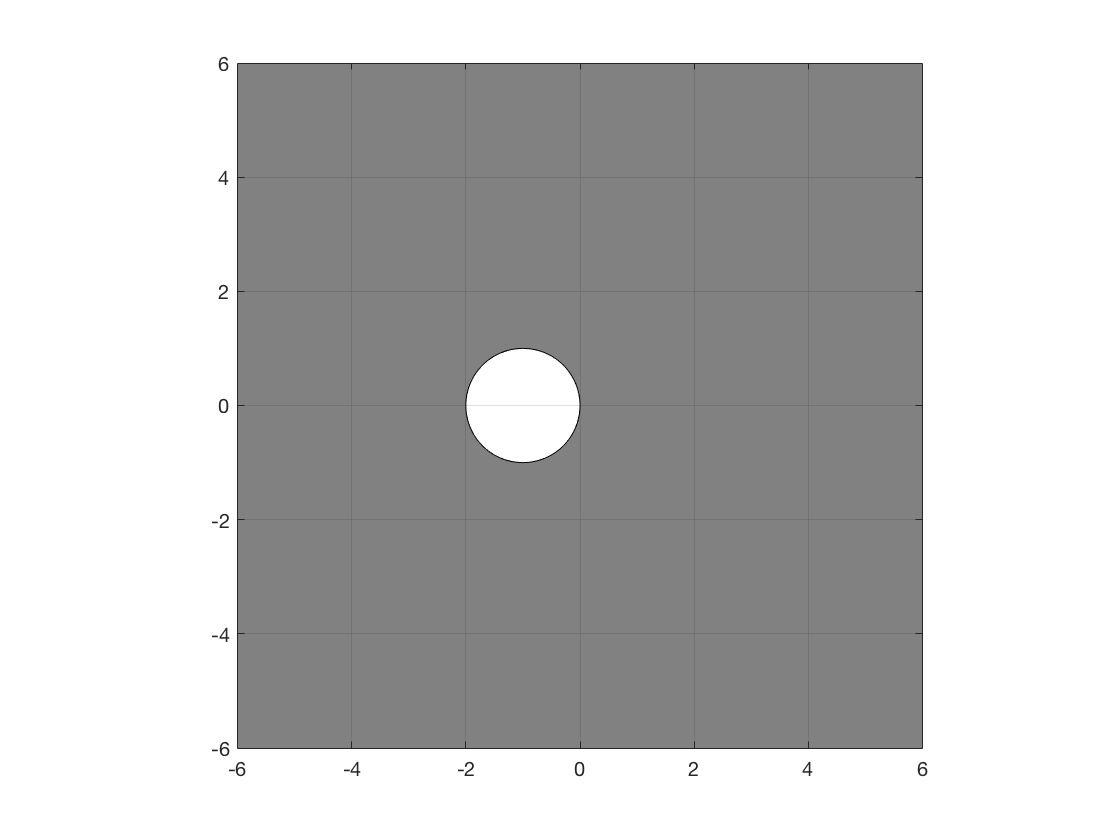
\includegraphics[width=\linewidth]{EE.png}
			\vspace{-5ex} 
			\caption*{Explicit Euler}
		\end{subfigure}%%
		\begin{subfigure}[b]{0.25\linewidth}
			\centering
			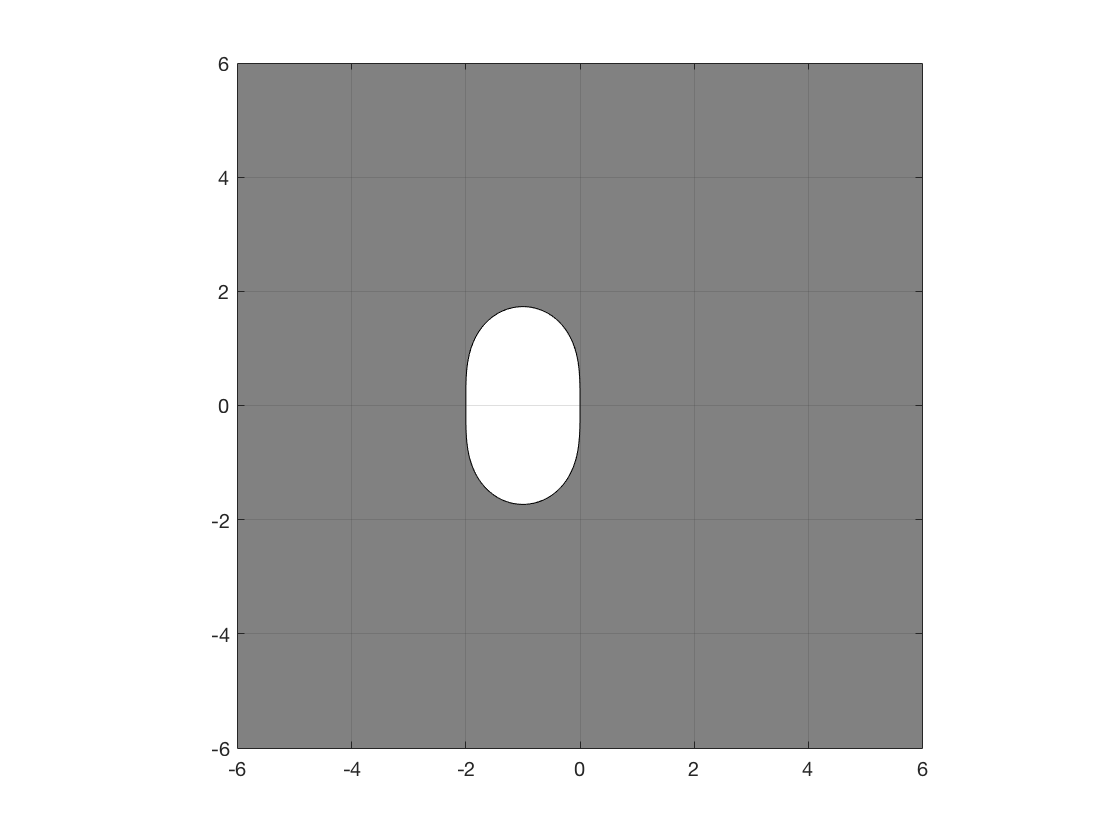
\includegraphics[width=\linewidth]{RK2.png} 
			\vspace{-5ex}
			\caption*{RK2}
		\end{subfigure}%%
		\begin{subfigure}[b]{0.25\linewidth}
			\centering
			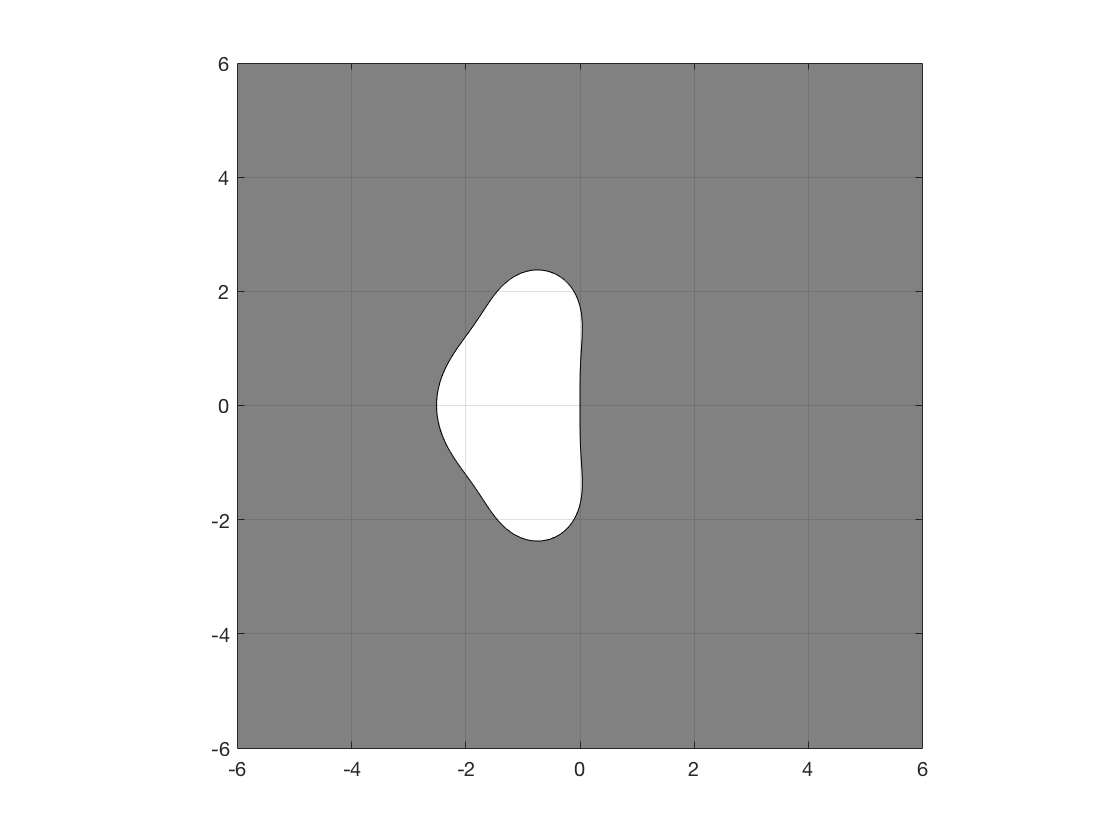
\includegraphics[width=\linewidth]{RK3.png} 
			\vspace{-5ex}
			\caption*{RK3}
		\end{subfigure}%%
		\begin{subfigure}[b]{0.25\linewidth}
			\centering
			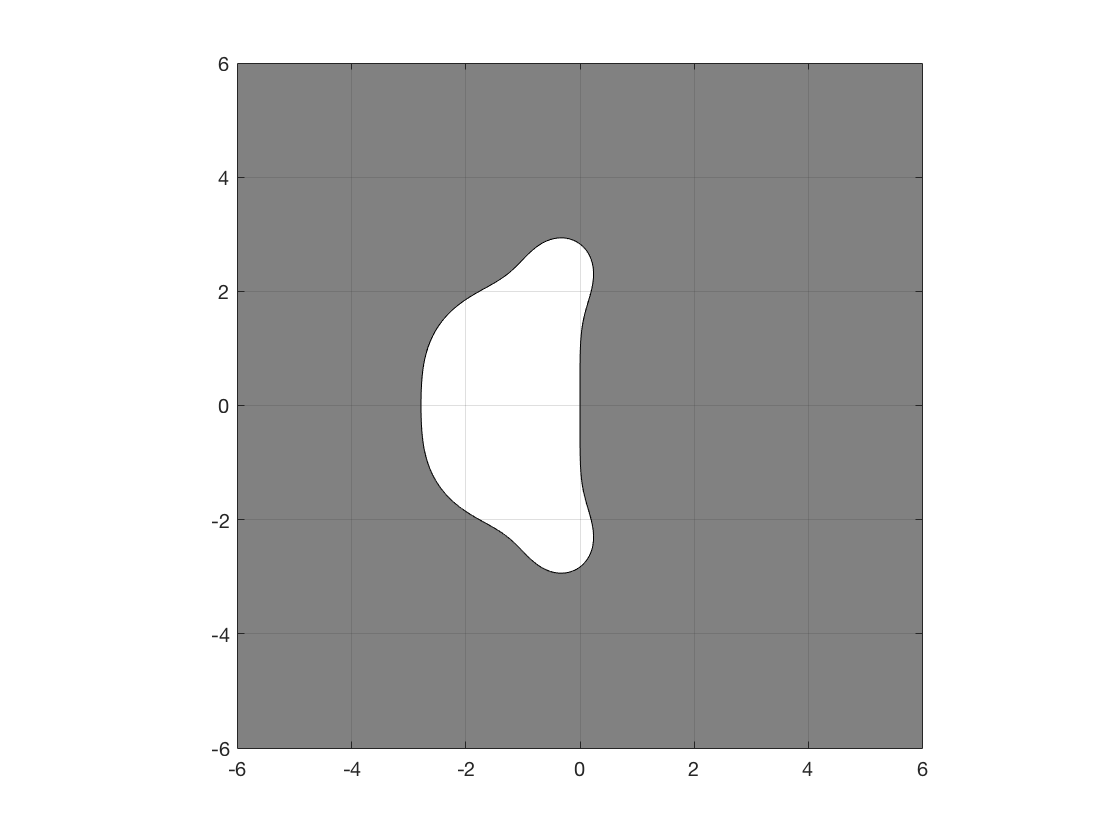
\includegraphics[width=\linewidth]{RK4.png} 
			\vspace{-5ex}
			\caption*{RK4}
		\end{subfigure}\\
		\begin{subfigure}[b]{0.25\linewidth}
			\centering
			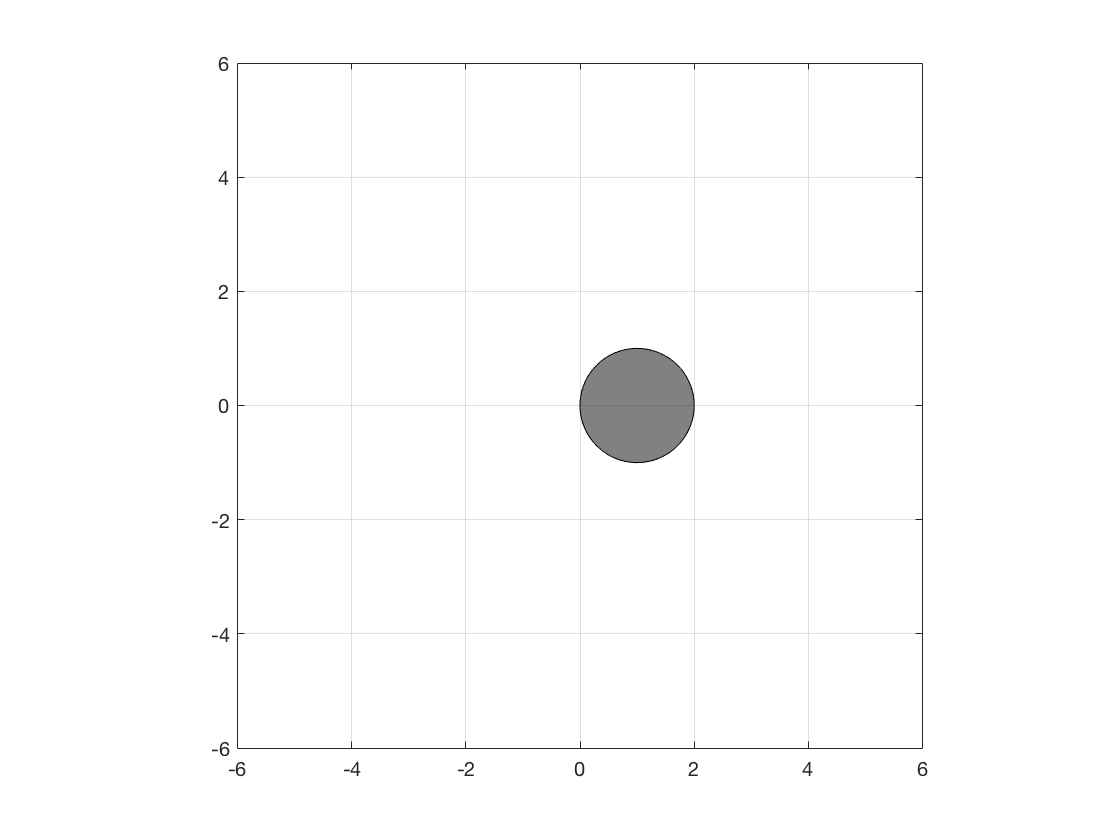
\includegraphics[width=\linewidth]{IE.png} 
			\vspace{-5ex}
			\caption*{Implicit Euler}
		\end{subfigure}%%
		\begin{subfigure}[b]{0.25\linewidth}
			\centering
			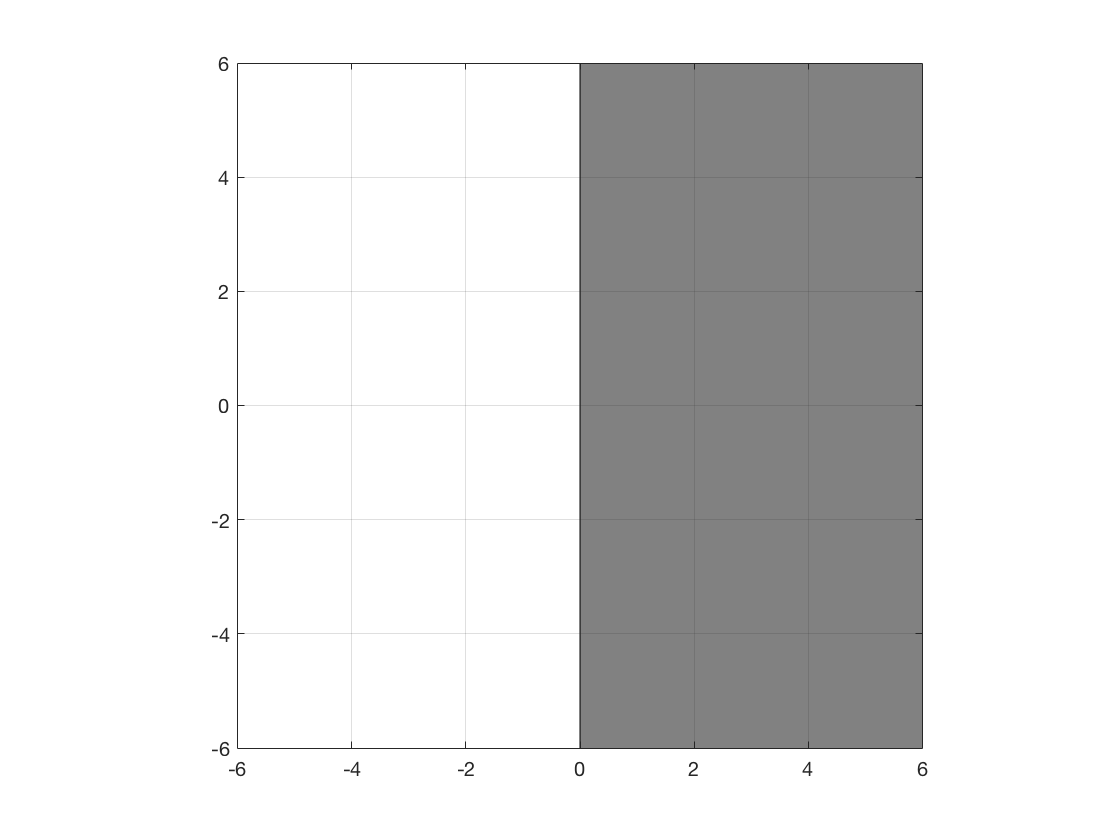
\includegraphics[width=\linewidth]{TR.png} 
			\vspace{-5ex}
			\caption*{Trapezoidal Rule/AM2}
		\end{subfigure}%%
		\begin{subfigure}[b]{0.25\linewidth}
			\centering
			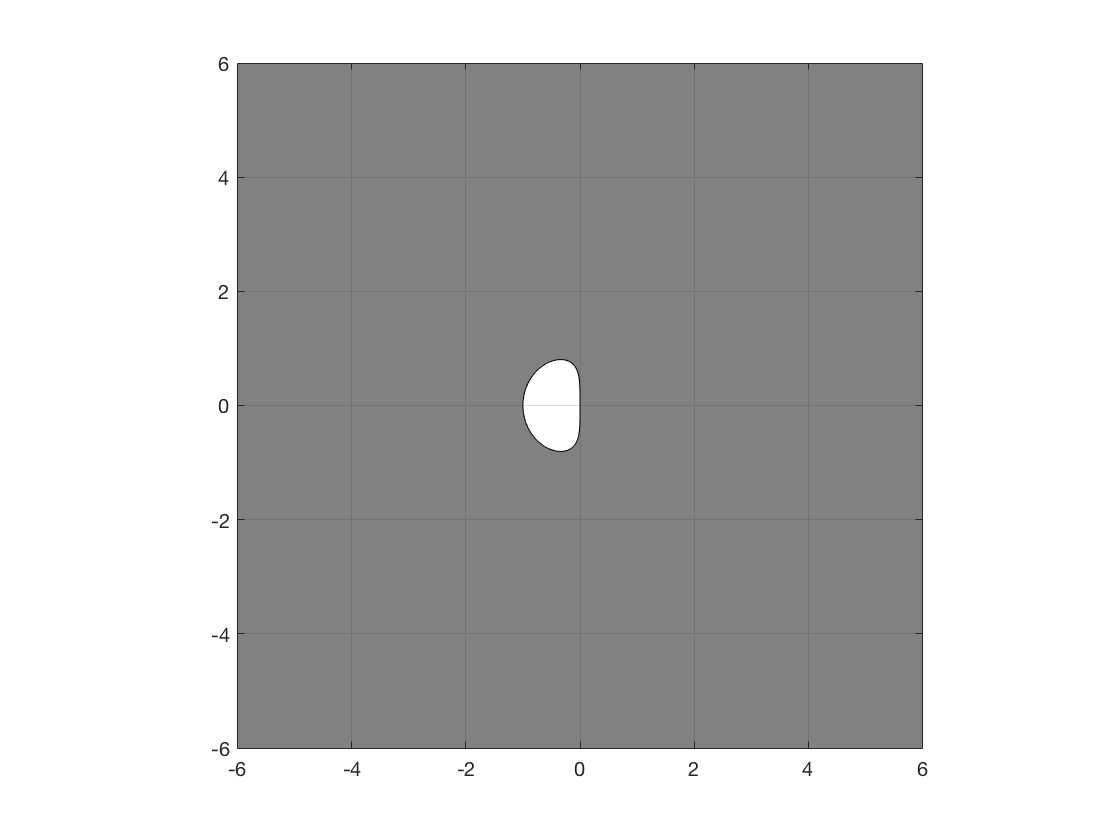
\includegraphics[width=\linewidth]{AB2.png} 
			\vspace{-5ex}
			\caption*{AB2}
		\end{subfigure}%%
		\begin{subfigure}[b]{0.25\linewidth}
			\centering
			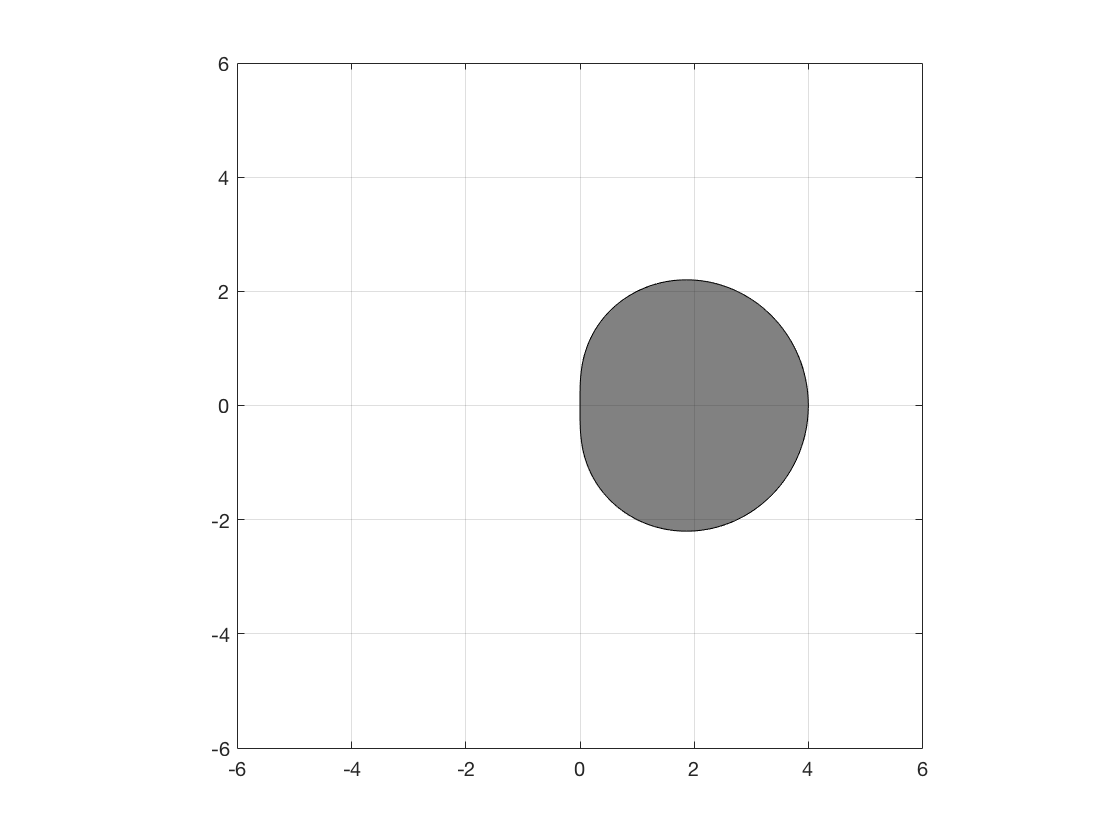
\includegraphics[width=\linewidth]{BDF2.png} 
			\vspace{-5ex}
			\caption*{BDF2}
		\end{subfigure} 
	\end{figure}
	The white space above is the stability region. The stability polynomials are listed below:
	\begin{itemize}
		\item 
		Explicit Euler: $\phi(z) = 1 + z$
		\item 
		RK2: $\phi(z) = 1 + z + \frac{1}{2}z^2$
		\item 
		RK3: $\phi(z) = 1 + z + \frac{1}{2}z^2 + \frac{1}{6}z^3$
		\item 
		RK4: $\phi(z) = 1 + z + \frac{1}{2}z^2 + \frac{1}{6}z^3 + \frac{1}{24}z^4$
		\item 
		Explicit Euler: $\phi(z) = \frac{1}{1-z}$
		\item 
		Trapezoidal Rule/AM2: $\phi(z) = \frac{1+z/2}{1-z/2}$
		\item 
		AB2: $\phi(z) = (2+3z\pm\sqrt{9z^2+4z+4})/4$
		\item 
		BDF2: $\phi(z) = \frac{-2\pm\sqrt{2z+1}}{2z-3}$
	\end{itemize}
	The implicit methods have larger stability regions than the explicit methods do. Implicit Euler, trapezoidal rule and BDF2 are  A-stable, while the ERK methods are not A-stable.
\end{enumerate}

\end{document}
